\capitulo{3}{Conceptos teóricos}

El proyecto cubre todo el proceso de creación de la aplicación, desde el diseño, implementación del código, hasta el despliegue de la misma en la \emph{Play Store}. Para ello se ha tenido que realizar un proceso de búsqueda para determinar que herramientas, lenguajes de programación, entornos de desarrollo son los más apropiados para un despliegue ágil.

Todo esto se sitúa en un mercado altamente competitivo, con una gran variabilidad (usuarios, empresas, desarrolladores ...) y con un constante cambio. 

\section{Aplicaciones nativas}
Estas se denominan así porque se desarrollan en el lenguaje nativo de cada uno de los sistemas operativos. Dependiendo de la plataforma en la que se desee crear esta nueva aplicación requerirá conocer un lenguaje de programación y un entorno de desarrollo en concreto. A continuación se muestra una tabla~\ref{table:nativos} con las herramientas y lenguajes nativos:

\begin{table}[H]
	\begin{center}
		\begin{tabular}{ccc}
			\hline
			Sistema Operativo                        & Lenguaje Programación & Entorno \\ \hline
			Android				    & Java      & Android Studio					\\
			iOS			    & Objetive C, Swift       & Xcode						\\ \hline
		\end{tabular}
		\caption{Herramientas y lenguaje nativos}
		\label{table:nativos}
	\end{center}
\end{table}

Las ventajas principales son: están desarrolladas directamente sobre la capa nativa del dispositivo, el rendimiento será óptimo y todas las funcionalidades y características estarán disponibles desde el primer momento.

Entre las desventajas: el elevado coste y mantenimiento, ya que requiere personal más especializado, con mayor tiempo destinado al desarrollo. Pero el mayor inconveniente lo encontramos en que el código nativo de una plataforma no puede ser reutilizado para la otra. Algo que los frameworks actuales están empezando a ofrecer.

\section{Aplicaciones híbridas mediante Framework}
Un framework (término de origen anglosajón: marco de trabajo)~\cite{wiki:framework}, es una estructura conceptual y tecnológica de soporte definido, normalmente por módulos de software concretos, que sirve de base para la organización y el desarrollo de software. Las ventajas que ofrece son varias, entre las que se puede destacar:

\begin{itemize}
	\item \textbf{Único código fuente}: desarrollo de aplicaciones multiplataforma con un único lenguaje, reduciendo los costes de creación, mantenimiento y recursos destinados. Actualmente no todos los frameworks ofrecen esto, pero en la gran mayoría sí que se está integrando, ya que existe una gran lucha por la competitividad.
	\item \textbf{Evita repetición de código:} las partes más usadas, pasan a ser algo del \emph{core} del framework o simplemente que se pueden reutilizar fácilmente. 
	\item \textbf{Uso de buenas prácticas:} están basados en patrones de diseño que nos obligan a usar.
	\item \textbf{Elementos avanzados integrados:} dispone de librerías nativas que ofrecen \emph{Widgets} o funcionalidades de gran calidad, que llevan mucho tiempo implementar, o que la creación de los mismo desde cero, no llegaría a obtener una calidad del mismo nivel.
	\item \textbf{Desarrollo ágil:} por los factores anteriores, podemos centrarnos más en la lógica de negocio de la aplicación que se desea hacer de una manera más rápida y segura.
\end{itemize}

Por lo tanto, es necesario trabajar mediante frameworks, ya que nos garantiza una aplicación de mayor calidad que si la hacemos en código nativo.

\subsection{Opciones disponibles}
En el mercado existen muchos frameworks disponibles para el desarrollo de aplicaciones móviles, por lo que decantarse por uno no es tarea sencilla, ya que cada uno tiene sus pros y contras. En una encuesta realizada a mediados del 2019 en el siguiente foro: Forocohes~\cite{foro:encuesta}, uno de los más recomendados era Flutter, como se puede ver en la imagen~\ref{fig:encuesta}:

\begin{figure}[h]
	\centering
	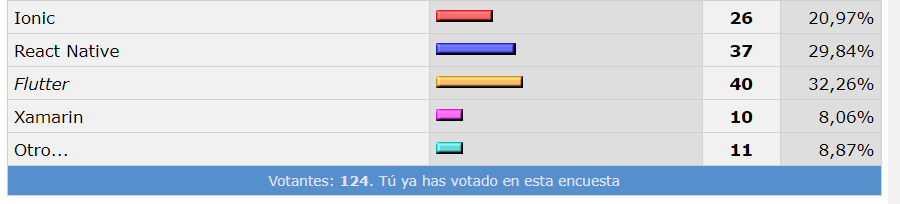
\includegraphics[width=1\textwidth]{teoria/encuesta.png}
	\caption{Encuesta en Forocoches}\label{fig:encuesta}
\end{figure}

Uno de los objetivos a la hora de encontrar el framework con el que hacer la aplicación, es que abarque el mayor número de dispositivos y usuarios. Es decir, que sea un framework \emph{crossplatform} o multiplataforma .

\subsubsection{Ionic}
Ionic~\cite{wiki:ionnic} se basa en lenguaje de programación javascript, html y css. Internamente esta basado en otro framework, como es Angularjs. La licencia es Open source, fue lanzado en el 2013 y permite el desarrollo para iOS y Android. A sufrido gran cantidad de cambios desde entonces.

Ventajas:
\begin{itemize}
	\item Una amplia comunidad de usuarios.
	\item Documentación extensa y de calidad.
\end{itemize}

Algunas de las desventajas:
\begin{itemize}
	\item Rendimiento algo menor, ya que no se desarrolla de forma nativa.
	\item Bibliotecas en constante cambio y evolución, más que ser algo bueno, puede que deje a la aplicación fuera de versión y se tenga que hacer otra vez.
\end{itemize}

\subsubsection{React native}
React native~\cite{wiki:react} fue creado en 2015 de la mano de Facebook. La licencia que tiene es MIT. La diferencia que tiene con React original, es que no manipula el DOM, por lo que tampoco usa HTML o CSS. 
Se programa en javascript. Las aplicaciones más conocidas que usan este framework son Instagram y Facebook.

Ventajas:
\begin{itemize}
	\item Gran comunidad de usuarios y herramientas.
	\item Mejora de las funcionalidades constantemente.
\end{itemize}

Algunas de las desventajas:
\begin{itemize}
	\item Rendimiento algo menor.
	\item No es código nativo, pero casi, por lo que no tiene soporte oficial de Google y Apple.
\end{itemize}

\subsubsection{Xamarin}
Xamarin~\cite{wiki:xamarin} creado por Microsoft en el 2011, por lo que está desarrollado en .NET, siendo propietario.

Ventajas:
\begin{itemize}
	\item Permite el desarrollo de iOS, Android, web y nativas de escritorio.
	\item Puede llamar a fragmentos de código en otros lenguajes usados en otras plataformas.
	\item Soporte para wearables.
\end{itemize}

Algunas de las desventajas:
\begin{itemize}
	\item Acceso limitado a las bibliotecas.
	\item El soporte es escaso y las actualizaciones son poco frecuentes.
	\item Comunidad grande pero pequeña comparada con otras.
	\item Aplicaciones de mayor tamaño.
	\item Mayor coste que otras.
\end{itemize}

\subsubsection{Otros}
Hay muchos otros, como kotlin, Apache Cordoba, jQuery Mobile, Native script...
Pero no me convencieron por diversas razones, como la curva de aprendizaje, costes, dificultades técnicas, entre otras.
 
\section{Flutter}
Flutter~\cite{wiki:flutter} es un SDK de código abierto creado por Google a finales del 2018. Permite que los desarrolladores puedan crear aplicaciones para iOS, Android y web.

Se encuentra escrito en Dart, que es un lenguaje de programación creado por Google en 2011. Pretende conseguir una mejora del lenguaje javascript, pero sin querer sustituirlo. Es decir, ofrecer mejores resultados y alternativas para algunos problemas, siendo una herramienta de mayor calidad para proyectos más grandes y que necesitan un desarrollo veloz.

Flutter es una herramienta muy reciente, con la que se pueden hacer aplicaciones comerciales para varias plataformas sin tener que programar exclusivamente para cada una de ellas. Ya que nos ofrece la compilación nativa directamente, reduciendo los costes a la hora de tener que llevar proyectos en los que sea necesario estar varias plataformas.

Las características más importantes son: 

\begin{itemize}
	\item Desarrollo rápido de las aplicaciones. Cuando se dice rápido es porque permite \emph{hot reload}. Lo que significa carga en caliente durante la fase de desarrollo. Implica que no es necesario tener que compilar todo el código, si no aquellas partes que fueron modificadas. Lo que permite en tiempo de ejecución ver los cambios.
	\item Está muy optimizado, con una evolución y soporte constante.
	\item Es un lenguaje de programación respaldado por Google, con lo que esto conlleva. Seguridad, confianza, fiabilidad, soporte, cursos y un montón de herramientas (más de 300 apis distintas: mapas, reconocimiento facial, traductor ...).
	\item La integración con el sistema operativo Android es mucho más eficaz, ya que este también pertenece a Google.
	\item Cuando se compila lo hace a nativo, ofreciendo una ganancia de rendimiento.
	\item La curva de aprendizaje es baja, en el caso de que sepamos javascript, typescript o ecmascript. Pero en caso contrario, no es especialmente empinada.
	\item La calidad de las animaciones y transiciones.
\end{itemize}

Las desventajas que tiene son:
\begin{itemize}
	\item La mayor parte de la documentación se encuentra en inglés, pero es más problema del desarrollador, que de la propia documentación del framework.
	\item Las aplicaciones ocupan más espacio que las nativas, ya que suelen incluir el SDK al completo.
	\item Al ser tan nuevo, tiene algunos problemas, no ofrece todas las funcionalidades, como las que tienen otras plataformas. Google lo sabe y está trabajando mucho en ello.
	\item Es una comunidad pequeña, pero ha crecido en dos años más que otras en tiempos similares.
\end{itemize}

Al final me decanté por este Framework básicamente porque es algo nuevo y disruptivo. El respaldo de Google se me presentaba como garantía, con la tranquilidad que eso conlleva. Es decir, todo el \emph{cloud services de Google} se puede integrar con gran facilidad.
Otra de las cosas que me incentivaron a elegirlo es que la comunidad lo a recibido con los brazos abiertos, como se puede ver en la encuesta~\ref{fig:encuesta} anterior, se encuentra entre los favoritos de los desarrolladores.

\subsection{Firebase}
Firebase~\cite{wiki:firebase} es una plataforma para el desarollo de aplicaciones web, Android e iOS, creada por Google en el 2014. Esta en la nube, formando el \emph{Google Cloud Plataform}, que consta de un conjunto de herramientas para dotar de una calidad enorme a los proyectos. Ya que permite la integración del ecosistema de Google como un todo.

Fue integrada en el proyecto por el hecho de ser un servicio gratuito y que aportaba gran valor a la aplicación. Firebase pasa a ser de pago cuando la app tiene que escalarse a un nivel más grande, por el crecimiento en número de usuarios o la gran cantidad de peticiones que se realicen a la misma. Algunas de las herramientas que integra son de pago, otras no.

Por lo tanto al ser multiplataforma es un backend con el que poder controlar todo, ganancias, gastos, escalabilidad, nuevos productos, herramientas... 

Entre los servicios que ofrece destacan entre otros:

\begin{itemize}
	\item \textbf{Real Time Data Base:} base de datos simples en tiempo real, si fuera necesario tener que guardar música, video o fotos, tiene otra parte dedicada a ficheros llamada \emph{Storage}.
	\item \textbf{Crash reporting:} herramienta para el reporte de errores que se producen en la aplicación.
	\item \textbf{Autentication:} integración con la mayor cantidad de aplicaciones de redes sociales en las que su API permite la identificación de usuarios. Obviamente el propio Google es una de ellas. Lo podemos ver en la siguiente imagen~\ref{fig:inicio}:
	\begin{figure}[H]
		\centering
		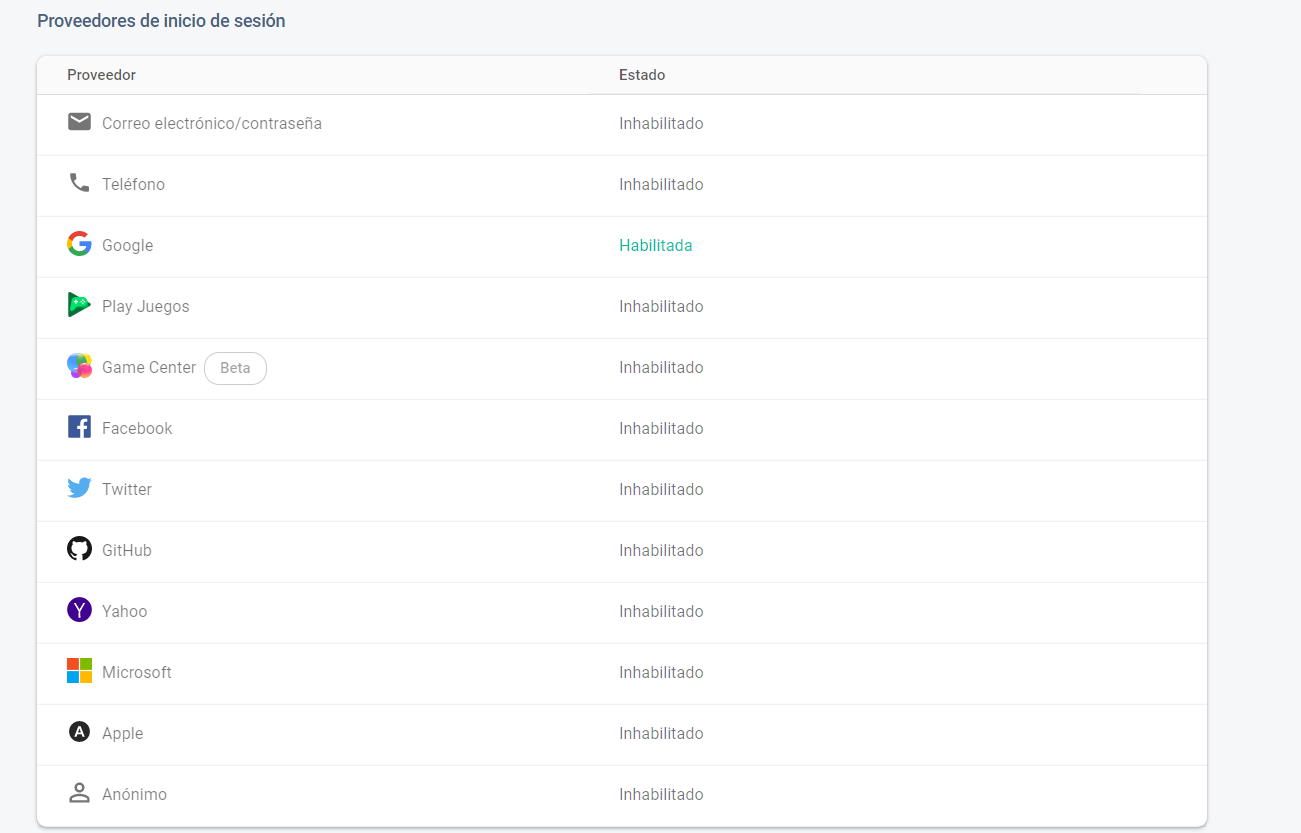
\includegraphics[width=1\textwidth]{teoria/inicio.png}
		\caption{Inicio de sesión}\label{fig:inicio}
	\end{figure}
	\item \textbf{Test lab:} probar la aplicación antes de realizar el despliegue de la misma. También el lanzamiento de pruebas alfa y beta.
	\item \textbf{Remote config:} hacer cambios internos del funcionamiento de la aplicación sin tener que recomplilar o actualizar.
	\item \textbf{Hosting:} servidor donde se puede publicar una página web.
	\item \textbf{Análisis:} mediante las analíticas que ofrece~\ref{fig:numerousers}, sirve como herramienta de toma de decisiones. Pudiendo optimizar a que mercados dirigirse mediante una estrategia de marketing.
	\begin{figure}[H]
		\centering
		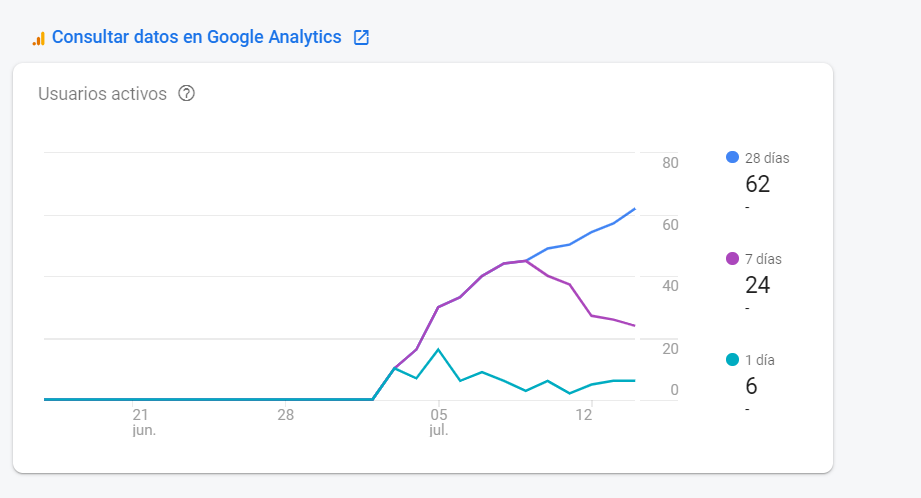
\includegraphics[width=1\textwidth]{teoria/numerousers.png}
		\caption{Ejemplo de Analytics}\label{fig:numerousers}
	\end{figure}
\end{itemize}
